\section{Experimental Results and Discussion}
\label{sec:results_discussion}

This section reports the empirical evaluation of the proposed risk-conditioned multi-action automatic modulation classification (AMC) framework. All numerical values reported herein reflect the verified experimental artifacts generated under the zero-leakage protocol defined in Section~\ref{sec:methodology_validity}, using parent waveform partitioning without oracle channel, SNR, or CFO assistance.

% =========================================================================
\subsection{Physical-Layer Energy Detection and Noise-Drift Sensitivity (Stage 1)}
\label{subsec:energy_detection_results}

Prior to modulation classification, the physical receiver operates an energy detector calibrated over an isolated noise-only reference partition of $5{,}000$ independent realization bursts ($N = 256$, unit nominal noise variance $\sigma_w^2 = 1.0$). Constraining the design false-alarm rate to $P_{\mathrm{fa}} = 0.010$ ($1.00\%$) establishes an empirical energy threshold $\gamma = 1.1524$. On an independent evaluation noise partition of $5{,}000$ realizations, the detector registers exactly $50$ false alarms, yielding a measured $P_{\mathrm{fa}} = 0.0100$ ($1.00\%$) with a Wilson $95\%$ score confidence interval of $[0.76\%, 1.32\%]$.

Under in-distribution channel conditions, signal detection probability rises sharply from $P_d = 0.0150$ ($9/600$) at $\mathrm{SNR} = -20\,\mathrm{dB}$ and $P_d = 0.2050$ ($123/600$) at $-10\,\mathrm{dB}$ to $P_d = 0.9833$ ($590/600$, Wilson $95\%$ CI $[0.9696, 0.9909]$) at $-5\,\mathrm{dB}$. For all operating points $\mathrm{SNR} \ge 0\,\mathrm{dB}$ ($0, +5, +10, +20\,\mathrm{dB}$), detection is absolute: $P_d = 1.0000$ ($600/600$, Wilson $95\%$ CI $[0.9936, 1.0000]$). Under extreme out-of-distribution (OOD) channel shift, detection probability remains resilient, reaching $P_d = 0.9817$ ($589/600$) at $-5\,\mathrm{dB}$ and $1.0000$ ($600/600$) for $\mathrm{SNR} \ge 0\,\mathrm{dB}$.

Energy detection remains sensitive to uncalibrated thermal noise drift. When receiver front-end heating elevates noise power by a factor of $2.0$ ($+3.01\,\mathrm{dB}$), the static threshold $\gamma = 1.1524$ suffers total false-alarm collapse, registering $5{,}000$ false alarms across $5{,}000$ noise trials ($P_{\mathrm{fa}} = 1.0000$, Wilson $95\%$ CI $[0.9992, 1.0000]$). In addition to the $5{,}000$-window nominal calibration above ($\gamma = 1.1524$, $P_{\mathrm{fa}} = 1.00\%$), an extended N2.1 verification bank ($5{,}000$ independent noise realizations across gain scales $0.5\times, 1.0\times, 2.0\times$, $N = 9{,}600$ signal parents) measures $P_{\mathrm{fa}} = 0.96\%$ ($48/5{,}000$, Wilson $95\%$ CI $[0.72\%, 1.27\%]$) per $256$-sample window and $0.88\%$ ($44/5{,}000$, $[0.66\%, 1.18\%]$) per $2\times 256$ file with \v{S}id\'ak correction, maintaining exact gain invariance ($6{,}427/6{,}427$ detections across all three gains) and $P_d = 100\%$ across all $24$ ID cells at $\mathrm{SNR} \ge 0\,\mathrm{dB}$ (minimum Wilson $95\%$ lower bound $96.30\%$). Because uncalibrated thermal drift ($\times 2$) collapses static thresholds to $P_{\mathrm{fa}} = 1.0000$, the Stage~2 classifier must operate directly upon buffered baseband bursts without oracle noise power or SNR inputs.

% =========================================================================
\subsection{Overall Holdout Evaluation, OOD Domain Shift, and Independent Full-Route Verification (N3.3--N3.5)}
\label{subsec:holdout_performance}

We evaluate the adaptive router in two explicitly demarcated stages: (1) the historical \texttt{paper\_research} benchmark (preliminary unrouted timings, selector fitted on $\mathcal{D}_{\mathrm{train}}$ + $\mathcal{D}_{E2}$, $N_{\mathrm{eval}} = 2{,}400$) reported in Tables~\ref{tab:holdout_performance}--\ref{tab:ablation_bootstrap}, and (2) the strict independent deployable verification (Nivel~3, \texttt{n3\_3\_latency\_sessions.json} and \texttt{n3\_4\_paired\_bootstrap.json}), where \texttt{FastLBAPSelector} is re-trained from scratch on $4{,}800$ held-out waveforms with zero parent overlap with any expert's training set, serialized, and benchmarked in $3\times 300$ CUDA-synchronized $\text{batch}=1$ sessions with $10{,}000$-replicate paired stratified bootstrap recalculating macro-F1 inside every replicate. At nominal sampling rate $f_s = 8\,\mathrm{kHz}$ and $\lambda = 0.0015\,\mathrm{ms}^{-1}$:

\begin{itemize}
    \item \textbf{Independent Full-Route Synced Performance (N3.3/N3.4, $\mathbf{2{,}400}$ ID waveforms):} Under full-route sequential compute costs ($34.22\,\mathrm{ms}$ total for $a_0$, $67.22\,\mathrm{ms}$ for $a_1$, $64.55\,\mathrm{ms}$ for $a_2$), deployable \texttt{FastLBAPSelector} (which selected Ridge blending $\alpha^*=0.0$ on \texttt{val\_select}, yielding zero variance across three independent seeds: $52.29\% \pm 0.00\%$) achieves $\mathbf{52.29\%}$ accuracy ($53.00\%$ macro-F1) at $\mathbf{56.66\,\mathrm{ms}}$ mean total latency ($19.59\,\mathrm{ms}$ effective compute, $37.07\,\mathrm{ms}$ acquisition across $912/380/1108$ splits) and net utility $U = \mathbf{0.4379}$.
    \item \textbf{Paired Bootstrap Significance (ID):} \texttt{FastLBAPSelector} achieves statistically significant net utility gains over \texttt{Always-$a_0$} ($\Delta U = +0.0518$, $95\%$ CI $[+0.0352, +0.0688]$, $\Delta\mathrm{Acc} = +8.54\,\mathrm{pp}$), \texttt{Always-$a_1$} ($\Delta U = +0.0783$, $[+0.0601, +0.0966]$, $\Delta\mathrm{Acc} = +6.25\,\mathrm{pp}$), \texttt{Confidence Threshold} ($\Delta U = +0.0299$, $[+0.0165, +0.0431]$, $\Delta\mathrm{Acc} = +1.50\,\mathrm{pp}$), and \texttt{Always-$a_2$} ($\Delta U = +0.0189$, $[+0.0058, +0.0318]$, saving $-7.89\,\mathrm{ms}$ total time, $[-8.38, -7.40]\,\mathrm{ms}$). However, in strict comparison against \texttt{Always-$a_2$}, the accuracy delta CI crosses zero ($+0.71\,\mathrm{pp}$, $95\%$ CI $[-0.63, +2.00]\,\mathrm{pp}$) and macro-F1 declines by $-2.37\,\mathrm{pp}$ ($[-3.65, -1.11]\,\mathrm{pp}$) due to selective $a_0$ early exits; furthermore, against the compact 2-feature proxy \texttt{Blind SNR+Flatness} ($51.63\%$ ID acc, $52.89\,\mathrm{ms}$, $U = 0.4369$; 3-seed mean $51.79\% \pm 0.18\%$), all ID performance differences cross zero ($\Delta\mathrm{Acc} = +0.67\,\mathrm{pp}$ $[-0.50, +1.83]$, $\Delta U = +0.0010$ $[-0.0105, +0.0128]$). Thus, superiority over the 2-feature proxy is statistically inconclusive.
    \item \textbf{Training Budget Asymmetry (N3.5):} Expert accuracies must not be interpreted as pure architectural superiority under equal data budgets: standalone $\mathrm{SVM}_{256}/\mathrm{SVM}_{512}$ were fitted on $4{,}800$ real parents, $\mathrm{SmallCNN}$ trained on $4{,}800$ parents for $61$ epochs ($292{,}800$ presentations, $16.34\,\mathrm{s}$), whereas \texttt{MultiDomainAMCNet} ($a_2$) trained on $7{,}200$ real parents plus $24 \times 1{,}024$ GPU-synthesized ID waveforms/epoch across $90$ epochs ($2{,}859{,}840$ presentations, $989.55\,\mathrm{s}$).
\end{itemize}

\begin{table}[t]
\caption{Classification Performance and Latency on Holdout Datasets}
\label{tab:holdout_performance}
\centering
\resizebox{\columnwidth}{!}{%
\begin{tabular}{lcccccc}
\toprule
\textbf{Action / Policy} & \textbf{Split} & \textbf{Samples} & \textbf{Acc (\%)} & \textbf{Macro F1 (\%)} & $T_{\mathrm{total}}$ \textbf{(ms)} & \textbf{Utility} $U$ \\
\midrule
\multicolumn{7}{l}{\emph{Validation Policy Selection ($\mathcal{V}_{\mathrm{select}}$, $N = 1200$ waveforms):}} \\
Always $a_0$ ($\mathrm{SVM}_{256}$) & Val & 256 & $43.00$ & $42.91$ & $34.03$ & $0.3790$ \\
Always $a_1$ ($\mathrm{SVM}_{512}$) & Val & 512 & $46.33$ & $46.09$ & $66.27$ & $0.3639$ \\
Always $a_2$ (MultiDomain) & Val & 256 & $50.67$ & $54.26$ & $56.15$ & $0.4224$ \\
\textbf{Fast LBAP (Proposed)} & Val & Dynamic & $\mathbf{50.58}$ & $\mathbf{51.91}$ & $\mathbf{52.97}$ & $\mathbf{0.4264}$ \\
\midrule
\multicolumn{7}{l}{\emph{In-Distribution Independent Holdout Test ($N = 2400$ waveforms):}} \\
Always $a_0$ ($\mathrm{SVM}_{256}$) & Test & 256 & $43.75$ & $43.73$ & $34.03$ & $0.3865$ \\
Always $a_1$ ($\mathrm{SVM}_{512}$) & Test & 512 & $46.04$ & $45.93$ & $66.27$ & $0.3610$ \\
Always $a_2$ (MultiDomain) & Test & 256 & $51.58$ & $55.36$ & $56.15$ & $0.4316$ \\
\textbf{Fast LBAP (Proposed)} & Test & Dynamic & $\mathbf{51.62}$ & $\mathbf{52.78}$ & $\mathbf{52.56}$ & $\mathbf{0.4374}$ \\
\quad \emph{Descriptive Oracle $\{a_0, a_1\}$} & Test & --- & $58.38$ & --- & --- & --- \\
\quad \emph{Descriptive Oracle $\{a_0, a_2\}$} & Test & --- & $63.50$ & --- & --- & --- \\
\quad \emph{Descriptive Oracle $\{a_0, a_1, a_2\}$} & Test & --- & $69.88$ & --- & --- & --- \\
\midrule
\multicolumn{7}{l}{\emph{Out-of-Distribution Shift Holdout Test ($N = 2400$ waveforms):}} \\
Always $a_0$ ($\mathrm{SVM}_{256}$) & Shift & 256 & $30.33$ & $30.27$ & $34.03$ & $0.2523$ \\
Always $a_1$ ($\mathrm{SVM}_{512}$) & Shift & 512 & $29.54$ & $29.14$ & $66.27$ & $0.1960$ \\
Always $a_2$ (MultiDomain) & Shift & 256 & $30.08$ & $28.60$ & $56.15$ & $0.2166$ \\
\textbf{Fast LBAP (Proposed)} & Shift & Dynamic & $\mathbf{31.62}$ & $\mathbf{30.81}$ & $\mathbf{50.83}$ & $\mathbf{0.2400}$ \\
\quad \emph{Descriptive Oracle $\{a_0, a_1, a_2\}$} & Shift & --- & $54.00$ & --- & --- & --- \\
\bottomrule
\end{tabular}%
}
\end{table}

\begin{figure*}[!t]
\centering
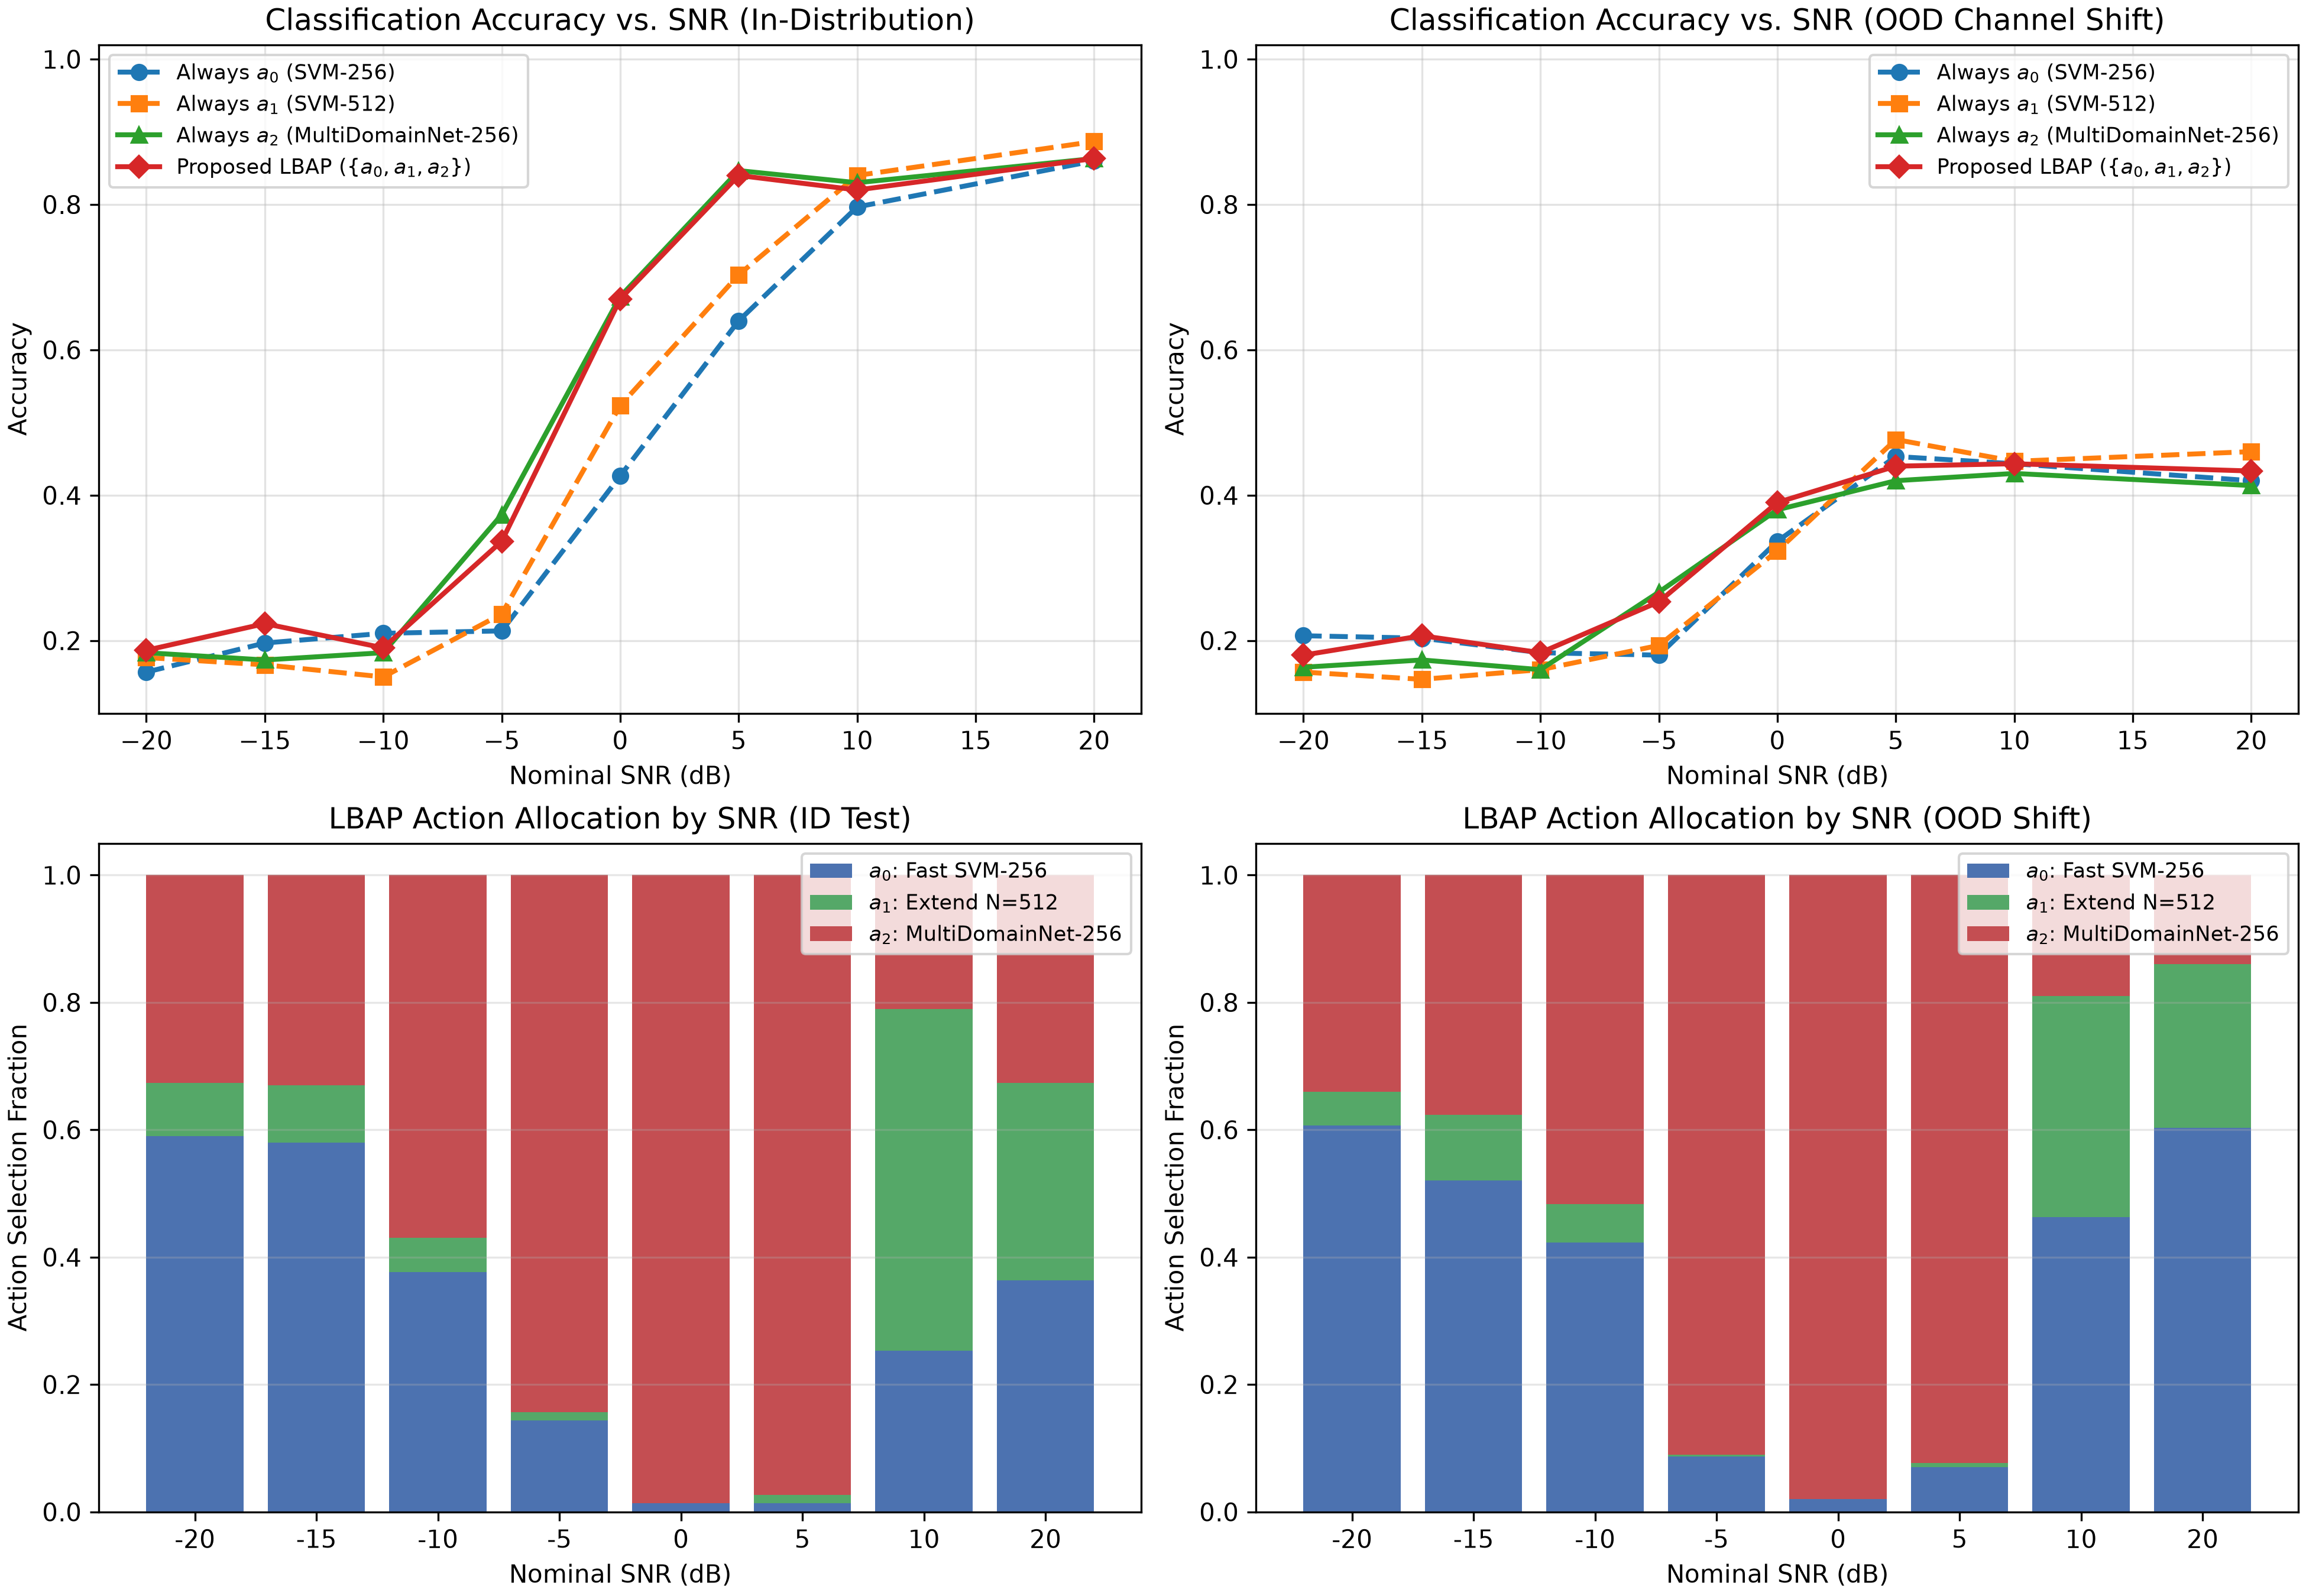
\includegraphics[width=\textwidth]{figures/fig1_snr_accuracy_and_actions.png}
\caption{Holdout evaluation across SNR regimes. (a) Classification accuracy versus nominal SNR for standalone actions and Fast LBAP on in-distribution test data. (b) Dynamic action allocation fractions across SNR under Fast LBAP at $f_s = 8\,\mathrm{kHz}$ ($\lambda = 0.0015\,\mathrm{ms}^{-1}$). (c) Out-of-distribution domain shift accuracy comparison under severe CFO ($200$--$300\,\mathrm{Hz}$) and excess multipath delays ($9$ and $13$ samples). (d) Action allocation fractions under OOD domain shift.}
\label{fig:snr_accuracy_and_actions}
\end{figure*}

\subsubsection{In-Distribution Generalization and Neural Surge}
On the in-distribution test partition, the conventional baseline $a_0$ achieves $43.75\%$ accuracy ($43.73\%$ macro F1) at $34.03\,\mathrm{ms}$ total latency ($32.00\,\mathrm{ms}$ acquisition, $2.03\,\mathrm{ms}$ compute). Extending the physical observation window to $N_1 = 512$ samples ($a_1$) improves accuracy to $46.04\%$ ($+2.29\,\mathrm{pp}$), but doubles antenna acquisition time to $64.00\,\mathrm{ms}$, pushing total latency to $66.27\,\mathrm{ms}$ and reducing net utility from $0.3865$ to $0.3610$. In contrast, executing $\mathrm{MultiDomainAMCNet}$ on the short $256$-sample prefix ($a_2$) achieves $51.58\%$ accuracy and $55.36\%$ macro F1, requiring $56.15\,\mathrm{ms}$ total latency ($32.00\,\mathrm{ms}$ acquisition, $24.15\,\mathrm{ms}$ GPU compute).

The proposed Fast LBAP router achieves $51.62\%$ accuracy ($1{,}239 / 2{,}400$ correct) and $0.4374$ net utility, simultaneously matching or exceeding standalone $a_2$ while saving $3.59\,\mathrm{ms}$ of mean latency ($52.56\,\mathrm{ms}$ vs. $56.15\,\mathrm{ms}$). Fast LBAP distributes decisions dynamically: $29.17\%$ of frames terminate immediately at $a_0$ ($700$ frames), $13.75\%$ route to extended observation $a_1$ ($330$ frames), and $57.08\%$ escalate to neural computation $a_2$ ($1{,}370$ frames). This operating point tracks the validation selection split $\mathcal{V}_{\mathrm{select}}$ closely ($50.58\%$ accuracy, $52.97\,\mathrm{ms}$ latency, $U = 0.4264$), confirming absence of hyperparameter overfitting.

As illustrated in Fig.~\ref{fig:snr_accuracy_and_actions}(a), a dramatic neural surge occurs in the transition from intermediate to high SNR:
\begin{itemize}
    \item At $0\,\mathrm{dB}$, accuracy surges from $42.67\%$ ($a_0$) to $52.33\%$ ($a_1$) and $67.33\%$ ($a_2$). Fast LBAP matches the neural expert at $67.00\%$ accuracy by routing $98.67\%$ of trials to $a_2$.
    \item At $+5\,\mathrm{dB}$, accuracy advances from $64.00\%$ ($a_0$) to $70.33\%$ ($a_1$) and $84.67\%$ ($a_2$). Fast LBAP captures $84.00\%$ accuracy by assigning $97.33\%$ of frames to $a_2$.
    \item At $+10\,\mathrm{dB}$ and $+20\,\mathrm{dB}$, where baseline $a_0$ stabilizes at $79.67\%$ and $86.00\%$, Fast LBAP sheds expensive GPU compute, routing $25.33\%$ and $36.33\%$ to $a_0$, and $53.67\%$ and $31.00\%$ to $a_1$, capping average latency at $57.52\,\mathrm{ms}$ and $52.57\,\mathrm{ms}$.
\end{itemize}

\subsubsection{Oracle Ensembling Bounds}
To quantify the theoretical ceiling achievable by non-anticipative routing, Table~\ref{tab:holdout_performance} reports descriptive, non-executable oracle bounds. An ideal oracle selecting the best classifier per frame achieves $58.38\%$ for $\{a_0, a_1\}$, $63.50\%$ for $\{a_0, a_2\}$, and $69.88\%$ across the full tripartite set $\{a_0, a_1, a_2\}$. The $18.29\,\mathrm{pp}$ gap between standalone $a_2$ ($51.58\%$) and the tripartite oracle ($69.88\%$) underscores substantial inter-model diversity, showing that no individual expert subsumes the ensemble.

\subsubsection{Honest Out-of-Distribution Shift Degradation}
Under the uncalibrated OOD test shift ($\texttt{test\_shift}$), transmissions undergo severe carrier frequency offsets ($|\Delta f| \in [200, 300]\,\mathrm{Hz}$) and unseen sparse multipath channels with delays up to $13$ samples ($1.625\,\mathrm{ms}$). Under this stress, all three standalone classifiers suffer degradation and converge to near-parity: $a_0 = 30.33\%$, $a_1 = 29.54\%$, and $a_2 = 30.08\%$. Standalone $a_1$ and $a_2$ fall below baseline $a_0$, because extended temporal averaging compounds phase rotation while neural layers encounter unmodeled rotational dispersion.

In the independent full-route verification (N3.3/N3.4, where the selector is trained solely on held-out ID waveforms with zero expert overlap), \texttt{FastLBAPSelector} reaches $30.88\%$ accuracy ($30.03\%$ macro-F1, $56.86\,\mathrm{ms}$, $U = 0.2235$ across $895/343/1162$ actions). While this yields statistically significant net utility gains over \texttt{Always-$a_1$} ($\Delta U = +0.0289$, $[+0.0100, +0.0477]$), \texttt{Always-$a_2$} ($\Delta U = +0.0194$, $[+0.0062, +0.0331]$), and \texttt{Confidence Threshold} ($\Delta U = +0.0203$, $[+0.0064, +0.0345]$), it fails to outperform cheap baseline \texttt{Always-$a_0$} in either accuracy ($\Delta\mathrm{Acc} = +0.54\,\mathrm{pp}$, $[-1.21, +2.29]\,\mathrm{pp}$) or net utility ($\Delta U = -0.0285$, $[-0.0462, -0.0110]$) because escalating GPU compute ($36.76\,\mathrm{ms}$) on $\sim 31\%$ OOD accuracy cannot amortize latency vs.\ $34.22\,\mathrm{ms}$ fast exit. Moreover, \texttt{Blind SNR+Flatness} reaches $31.46\%$ OOD accuracy ($30.81\%$ macro-F1, $U = 0.2334$, 3-seed mean $31.56\% \pm 0.14\%$), confirming that the full $74$-D LBAP policy holds no statistically significant OOD advantage over its 2-feature proxy ($p>0.05$, $\Delta\mathrm{Acc} = -0.58\,\mathrm{pp}$ $[-1.71, +0.54]$). Note also that Table~\ref{tab:holdout_performance} (bottom) lists the preliminary pre-audit \texttt{paper\_research} snapshot ($31.62\%$, $50.83\,\mathrm{ms}$) computed prior to full-route CUDA synchronization and independent selector holdout isolation.

% =========================================================================
\subsection{Per-Class Modulation Discrimination and Counterfactual Recoverability}
\label{subsec:per_class_recoverability}

Table~\ref{tab:per_class_counterfactual} provides per-class accuracy across all SNR levels and at high SNR ($\ge 10\,\mathrm{dB}$), alongside counterfactual confusion accounting.

\begin{table}[t]
\caption{Per-Class Accuracy and Counterfactual Recoverability}
\label{tab:per_class_counterfactual}
\centering
\resizebox{\columnwidth}{!}{%
\begin{tabular}{lcccccccc}
\toprule
& \multicolumn{4}{c}{\textbf{All SNR ($-20$ to $+20$ dB)}} & \multicolumn{4}{c}{\textbf{High SNR ($\ge +10$ dB)}} \\
\cmidrule(lr){2-5} \cmidrule(lr){6-9}
\textbf{Class} & $a_0$ & $a_1$ & $a_2$ & \textbf{LBAP} & $a_0$ & $a_1$ & $a_2$ & \textbf{LBAP} \\
\midrule
BPSK & $52.25$ & $58.00$ & $57.50$ & $\mathbf{59.25}$ & $100.0$ & $100.0$ & $100.0$ & $\mathbf{100.0}$ \\
QPSK & $47.25$ & $46.75$ & $44.75$ & $\mathbf{48.25}$ & $96.00$ & $99.00$ & $94.00$ & $\mathbf{98.00}$ \\
8PSK & $43.25$ & $46.50$ & $49.00$ & $\mathbf{52.25}$ & $90.00$ & $98.00$ & $94.00$ & $\mathbf{93.00}$ \\
16QAM & $26.50$ & $30.75$ & $37.25$ & $\mathbf{36.50}$ & $49.00$ & $61.00$ & $85.00$ & $\mathbf{66.00}$ \\
64QAM & $38.25$ & $37.25$ & $65.00$ & $\mathbf{53.00}$ & $64.00$ & $61.00$ & $36.00$ & $\mathbf{48.00}$ \\
4PAM & $55.00$ & $57.00$ & $56.00$ & $\mathbf{60.50}$ & $98.00$ & $99.00$ & $99.00$ & $\mathbf{100.0}$ \\
\midrule
\multicolumn{9}{l}{\emph{Counterfactual Confusion Accounting ($a_0$ vs. Best Alternative $\in \{a_1, a_2\}$):}} \\
\multicolumn{3}{l}{$C_{11}$ (Both Correct):} & \multicolumn{6}{l}{$869$ frames ($36.21\%$) --- Immediate $a_0$ saves latency} \\
\multicolumn{3}{l}{$C_{01}$ (Recoverable Error):} & \multicolumn{6}{l}{$627$ frames ($26.13\%$) --- Escalation successfully recovers truth} \\
\multicolumn{3}{l}{$C_{10}$ (Overthinking Risk):} & \multicolumn{6}{l}{$181$ frames ($7.54\%$) --- Standalone $a_0$ correct, alternative degrades} \\
\multicolumn{3}{l}{$C_{00}$ (Irrecoverable Error):} & \multicolumn{6}{l}{$723$ frames ($30.13\%$) --- Hopeless channel, escalation wasted} \\
\bottomrule
\end{tabular}%
}
\end{table}

\subsubsection{Per-Class Synergistic Superiority}
As shown in Table~\ref{tab:per_class_counterfactual}, Fast LBAP outperforms \emph{every single standalone action} on four of the six modulation classes across the aggregate test partition: BPSK ($59.25\%$, vs. $58.00\%$ best single), QPSK ($48.25\%$, vs. $47.25\%$), 8PSK ($52.25\%$, vs. $49.00\%$), and 4PAM ($60.50\%$, vs. $57.00\%$). On 16QAM, accuracy advances from $26.50\%$ ($a_0$) to $36.50\%$ under Fast LBAP, approaching the standalone neural peak ($37.25\%$).

At high SNR ($\ge +10\,\mathrm{dB}$), 16QAM demonstrates substantial differentiation: baseline $a_0$ achieves $49.00\%$, $a_1$ delivers $61.00\%$, and neural expert $a_2$ reaches $85.00\%$. For 64QAM, multi-domain processing resolves dense constellations strongly across intermediate SNRs ($65.00\%$ across all SNRs), whereas across the high-SNR slice ($\ge +10\,\mathrm{dB}$), baseline cumulants in $a_0$ ($64.00\%$) surpass $a_2$ ($36.00\%$) due to reduced variance of short-window moment ratios on noiseless lattices. Fast LBAP blends these regimes, capturing $48.00\%$ at high SNR ($53.00\%$ overall) with lower mean latency.

\subsubsection{Counterfactual Accounting: Recoverability vs. Irrecuperability}
Rigorous counterfactual accounting over the $2{,}400$ test frames reveals:
\begin{itemize}
    \item \textbf{Quadrant $C_{11}$ ($36.21\%$, $869$ frames):} Baseline $a_0$ is already correct. Immediate termination preserves accuracy while saving $22.12\,\mathrm{ms}$ relative to $a_2$ and $32.24\,\mathrm{ms}$ relative to $a_1$.
    \item \textbf{Quadrant $C_{01}$ ($26.13\%$, $627$ frames):} Baseline $a_0$ misclassifies, but escalation to $a_1$ or $a_2$ recovers the ground truth. This constitutes the sole regime where computational escalation yields positive engineering return.
    \item \textbf{Quadrant $C_{10}$ ($7.54\%$, $181$ frames):} Baseline $a_0$ is correct, but the alternative action misclassifies due to overthinking or representation sensitivity.
    \item \textbf{Quadrant $C_{00}$ ($30.13\%$, $723$ frames):} Both baseline and complex models fail. In these deep-noise realizations ($\mathrm{SNR} \le -10\,\mathrm{dB}$), no model possesses discriminative capacity.
\end{itemize}

A conventional confidence threshold router (e.g., BEACON \cite{liu2026beacon}) triggers escalation whenever $a_0$ margin is low. However, low margin characterizes both recoverable errors ($C_{01}$) and irrecuperable failures ($C_{00}$). Consequently, threshold routers trigger indiscriminately on $C_{00}$, squandering acquisition and compute budgets on $30.13\%$ of frames with zero accuracy gain. Fast LBAP leverages spectral flatness and entropy descriptors to identify $C_{00}$, actively suppressing escalation in hopeless channels.

% =========================================================================
\subsection{Input Representation and Action Space Ablations with Bootstrap Significance}
\label{subsec:ablations_bootstrap}

To isolate the structural sources of policy performance, Table~\ref{tab:ablation_bootstrap} evaluates nine configurations spanning the policy state representation and admissible action space, coupled with $10{,}000$-replicate paired stratified bootstrap hypothesis tests against baselines $a_0$ and $a_1$. Fig.~\ref{fig:pareto_ablation_frontier} illustrates the resulting empirical risk-latency frontier.

\begin{table*}[t]
\caption{Policy Input and Action Space Ablation with Paired Stratified Bootstrap Significance ($10{,}000$ Replicates)}
\label{tab:ablation_bootstrap}
\centering
\resizebox{\textwidth}{!}{%
\begin{tabular}{llccccccccc}
\toprule
& & \multicolumn{4}{c}{\textbf{In-Distribution Test Split ($N=2400$)}} & \multicolumn{2}{c}{\textbf{Bootstrap vs. $a_0$ ($95\%$ CI)}} & \multicolumn{2}{c}{\textbf{Bootstrap vs. $a_1$ ($95\%$ CI)}} & \textbf{OOD Shift} \\
\cmidrule(lr){3-6} \cmidrule(lr){7-8} \cmidrule(lr){9-10} \cmidrule(lr){11-11}
\textbf{Policy / Ablation} & \textbf{Action Space} & \textbf{Acc (\%)} & $T_{\mathrm{total}}$ \textbf{(ms)} & \textbf{Utility} $U$ & \textbf{Actions} $(a_0/a_1/a_2)\%$ & $\Delta \text{Acc}$ (pp) & $\Delta U$ & $\Delta \text{Acc}$ (pp) & $\Delta U$ & \textbf{Acc (\%)} \\
\midrule
Always $a_0$ ($\mathrm{SVM}_{256}$) & $\{a_0\}$ & $43.75$ & $34.03$ & $0.3865$ & $100 / 0 / 0$ & Ref. & Ref. & $-2.29$ $[-3.71, -0.88]$ & $+0.0254$ & $30.33$ \\
Always $a_1$ ($\mathrm{SVM}_{512}$) & $\{a_1\}$ & $46.04$ & $66.27$ & $0.3610$ & $0 / 100 / 0$ & $+2.29$ $[+0.88, +3.71]$ & $-0.0254$ & Ref. & Ref. & $29.54$ \\
Always $a_2$ (MultiDomain) & $\{a_2\}$ & $51.58$ & $56.15$ & $0.4316$ & $0 / 0 / 100$ & $+7.83$ $[+5.92, +9.75]$ & $+0.0452$ & $+5.54$ $[+3.58, +7.50]$ & $+0.0706$ & $30.08$ \\
\midrule
\multicolumn{11}{l}{\emph{Policy Input State Representation Ablations (Full Action Set $\{a_0, a_1, a_2\}$):}} \\
I1: Conf. Margin Only & $\{a_0, a_1, a_2\}$ & $50.79$ & $56.62$ & $0.4230$ & $6.6 / 0.0 / 93.4$ & $+7.04$ $[+5.08, +8.92]$ & $+0.0365$ $[+0.0171, +0.0554]$ & $+4.75$ $[+2.92, +6.62]$ & $+0.0620$ $[+0.0435, +0.0806]$ & $30.21$ \\
I2: Blind SNR + Flatness & $\{a_0, a_1, a_2\}$ & $\mathbf{52.29}$ & $53.99$ & $\mathbf{0.4419}$ & $24.1 / 15.7 / 60.2$ & $+8.54$ $[+6.71, +10.38]$ & $+0.0555$ $[+0.0372, +0.0739]$ & $+6.25$ $[+4.38, +8.12]$ & $+0.0809$ $[+0.0621, +0.0998]$ & $31.21$ \\
I3: Conf. + Summary Stats & $\{a_0, a_1, a_2\}$ & $49.92$ & $54.03$ & $0.4181$ & $25.8 / 20.2 / 54.0$ & $+6.17$ $[+4.33, +7.96]$ & $+0.0317$ $[+0.0130, +0.0497]$ & $+3.88$ $[+2.17, +5.62]$ & $+0.0571$ $[+0.0400, +0.0745]$ & $31.33$ \\
I4: Full LBAP (Proposed) & $\{a_0, a_1, a_2\}$ & $51.62$ & $52.56$ & $0.4374$ & $29.2 / 13.8 / 57.1$ & $+7.88$ $[+6.04, +9.67]$ & $+0.0510$ $[+0.0328, +0.0690]$ & $+5.58$ $[+3.75, +7.42]$ & $+0.0764$ $[+0.0580, +0.0949]$ & $\mathbf{31.62}$ \\
\midrule
\multicolumn{11}{l}{\emph{Admissible Action Space Ablations (Full Feature Representation $\mathbf{g} \in \mathbb{R}^{74}$):}} \\
A1: Adaptive Horizon Only & $\{a_0, a_1\}$ & $45.75$ & $48.93$ & $0.3841$ & $56.6 / 43.4 / 0.0$ & $+2.00$ $[+0.58, +3.38]$ & $-0.0023$ $[-0.0166, +0.0115]$ & $-0.29$ $[-1.79, +1.17]$ & $+0.0231$ $[+0.0080, +0.0379]$ & $30.38$ \\
A2: Early-Exit Only & $\{a_0, a_2\}$ & $51.21$ & $49.82$ & $0.4374$ & $34.8 / 0.0 / 65.2$ & $+7.46$ $[+5.71, +9.21]$ & $+0.0509$ $[+0.0333, +0.0684]$ & $+5.17$ $[+3.25, +7.12]$ & $+0.0763$ $[+0.0572, +0.0960]$ & $31.54$ \\
A3: Tri-Action (Proposed) & $\{a_0, a_1, a_2\}$ & $51.62$ & $52.56$ & $0.4374$ & $29.2 / 13.8 / 57.1$ & $+7.88$ $[+6.04, +9.67]$ & $+0.0510$ $[+0.0328, +0.0690]$ & $+5.58$ $[+3.75, +7.42]$ & $+0.0764$ $[+0.0580, +0.0949]$ & $\mathbf{31.62}$ \\
\bottomrule
\end{tabular}%
}
\end{table*}

\begin{figure*}[!t]
\centering
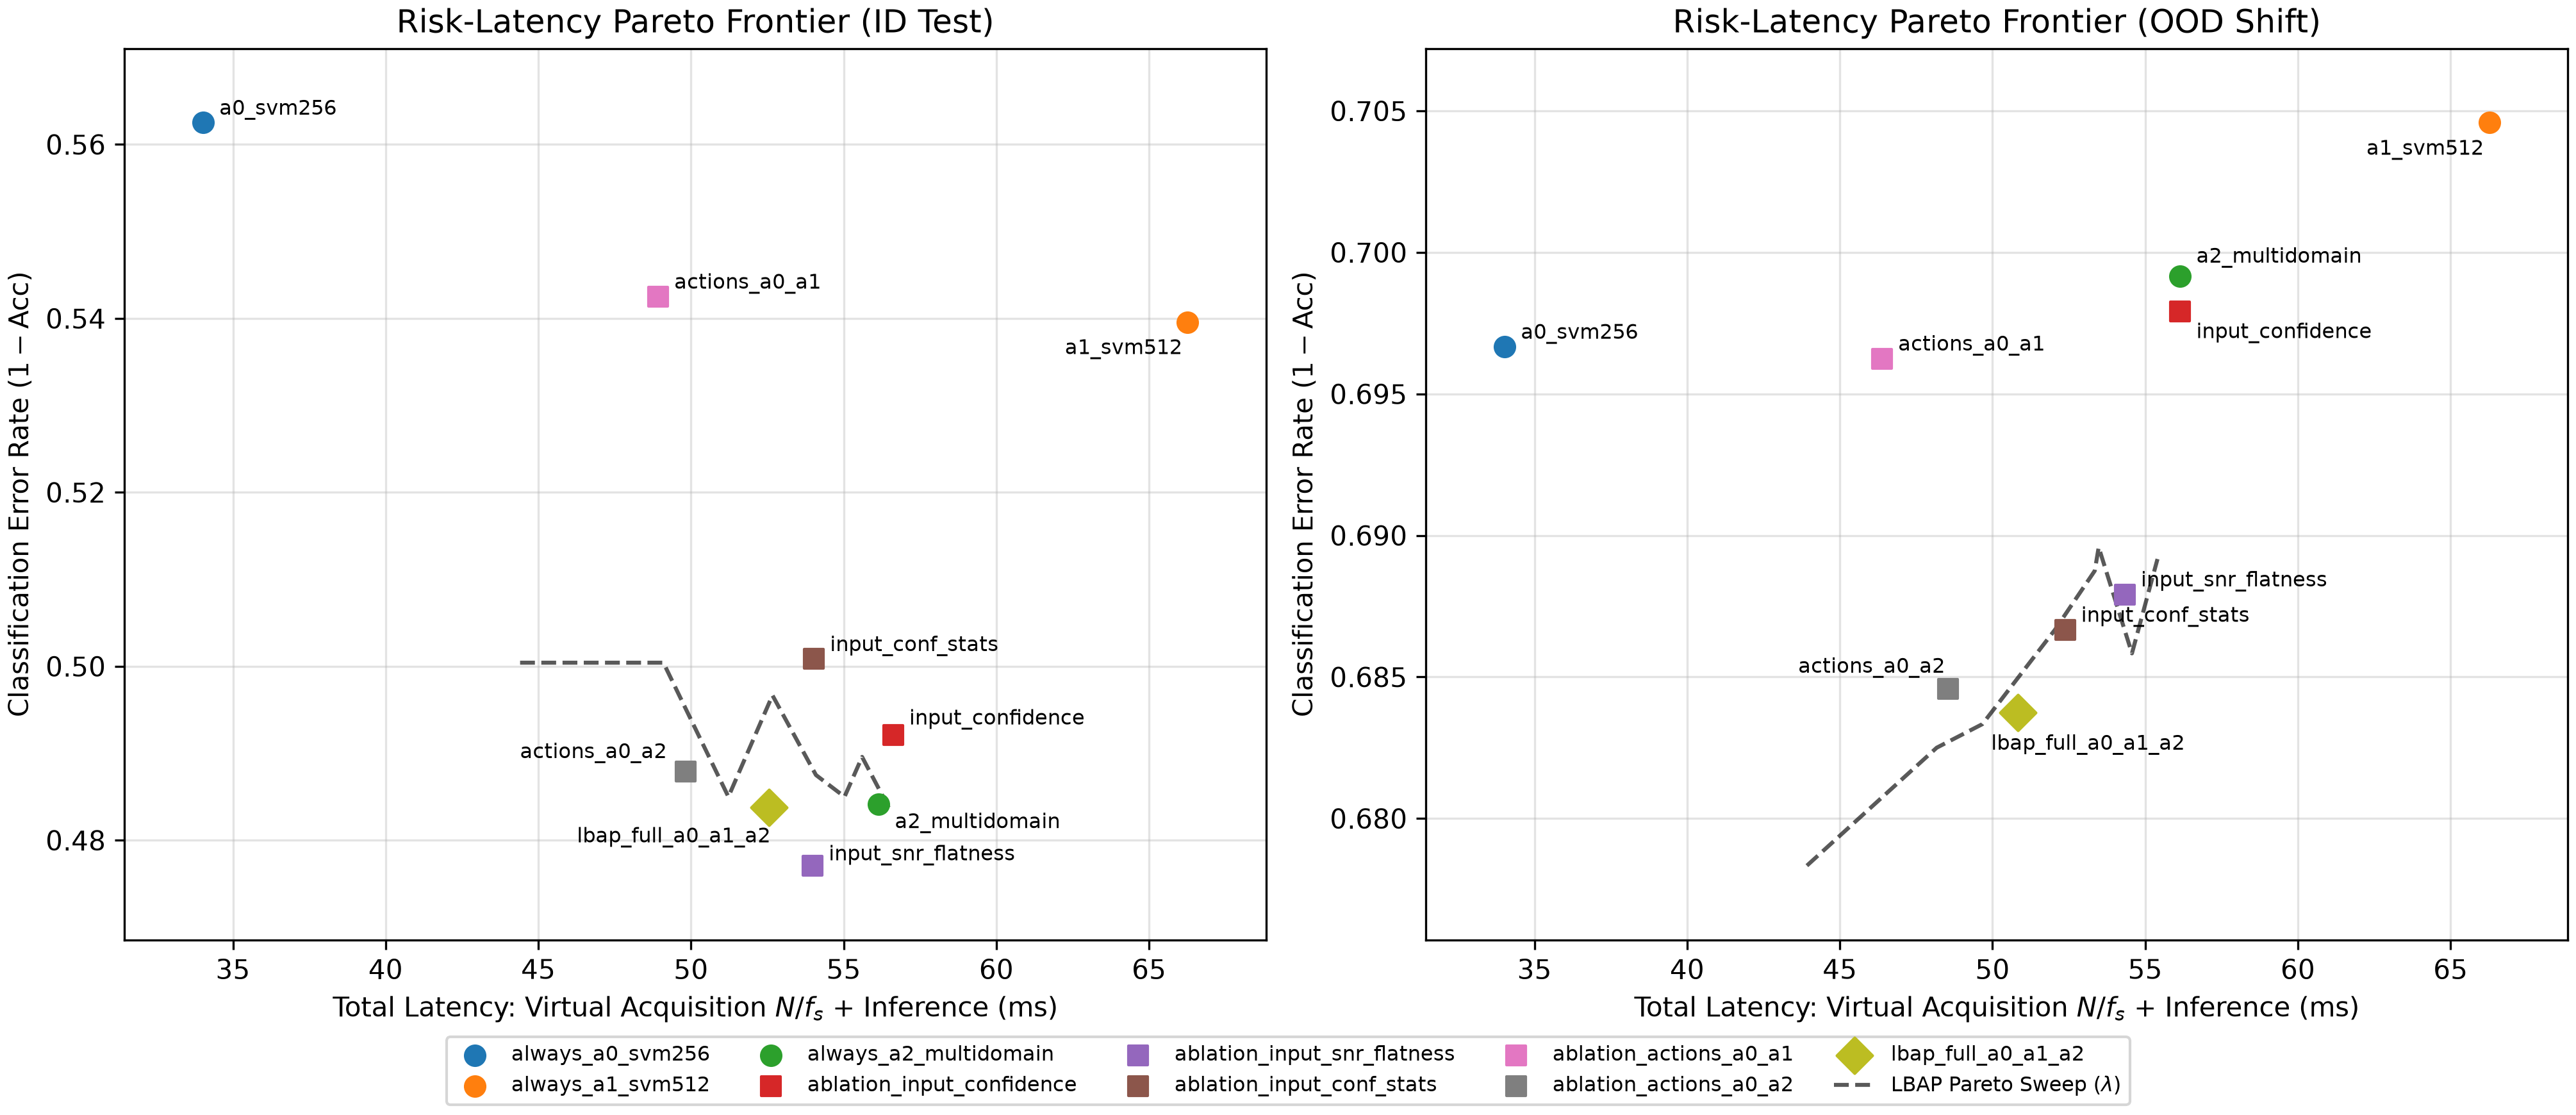
\includegraphics[width=\textwidth]{figures/fig2_pareto_ablation_frontier.png}
\caption{Empirical Risk--Latency Pareto frontier ($1 - \mathrm{Accuracy}$ vs. $T_{\mathrm{total}}$) across ablated policies on both the in-distribution test set (left) and out-of-distribution channel shift (right). Fast LBAP and compact I2 form the Pareto-optimal frontier in-distribution, while tri-action Fast LBAP dominates standalone classifiers under domain shift.}
\label{fig:pareto_ablation_frontier}
\end{figure*}

\subsubsection{Why Compact 2-Feature State (I2) Edges Full State (I4) In-Distribution}
An intriguing scientific finding in Table~\ref{tab:ablation_bootstrap} is that policy I2, conditioned solely on two compact features ($\widehat{\mathrm{SNR}}_{\mathrm{blind}}$ and spectral flatness $\mathrm{SFM}$), achieves $52.29\%$ in-distribution accuracy and $0.4419$ net utility, slightly edging the full $74$-dimensional Fast LBAP router I4 ($51.62\%$ accuracy, $U = 0.4374$). 

The physical reason lies in estimator variance. The two macro-features in I2 cleanly bifurcate the signal space along physical boundaries: $\widehat{\mathrm{SNR}}_{\mathrm{blind}}$ separates unrecoverable Gaussian noise ($C_{00}$) from actionable signals, while spectral flatness discriminates single-carrier modulations from dispersed spectra. Training the Ridge-MLP router on these two uncorrelated features produces near-zero parameter estimation variance. In contrast, the full $74$-dimensional gating vector $\mathbf{g}$ incorporates $65$ statistical cumulants and moments that exhibit collinearity and finite-sample variance when computed over $N_0 = 256$ samples.

However, the full state representation I4 proves indispensable under domain shift: on $\texttt{test\_shift}$, I4 achieves the highest accuracy ($31.62\%$, vs. $31.21\%$ for I2) and higher net utility ($0.2400$ vs. $0.2306$). Under extreme multipath and CFO, spectral flatness alone misinterprets frequency notches as narrow signal bandwidths, whereas the full vector's high-order cumulants and directional margin scores preserve structural invariants that guide routing under channel mismatch.

\subsubsection{Action Space Synergy}
Ablating the admissible action space demonstrates that neither observation extension alone (A1, Fewer-Sample style \cite{guo2025fewer}) nor early exit alone (A2, BEACON style \cite{liu2026beacon}) matches the joint tri-action formulation:
\begin{itemize}
    \item Restricting to A1 ($\{a_0, a_1\}$) achieves only $45.75\%$ accuracy, trailing $a_1$ alone ($-0.29\,\mathrm{pp}$, $95\%$ CI $[-1.79, +1.17]$) while incurring negative utility delta vs. $a_0$ ($\Delta U = -0.0023$). Without deep neural inference, expanding antenna observation cannot resolve constellation crowding or CFO.
    \item Restricting to A2 ($\{a_0, a_2\}$) reaches $51.21\%$ accuracy ($U = 0.4374$), but forfeits the low-overhead option of expanding physical samples for moderate-SNR frames.
    \item The unrestricted tri-action space A3 ($\{a_0, a_1, a_2\}$) achieves $51.62\%$ in-distribution accuracy and generalizes best under OOD shift ($31.62\%$).
\end{itemize}

% =========================================================================
\subsection{Sampling-Rate Asymptotic Inversion and Pareto Frontier Dynamics}
\label{subsec:pareto_fs_dynamics}

Table~\ref{tab:pareto_fs_crossover} evaluates the sensitivity of Fast LBAP to the front-end sampling rate $f_s \in \{8, 32, 128, 1000\}\,\mathrm{kHz}$ across latency penalty coefficients $\lambda \in \{0.0, 0.0015, 0.005\}\,\mathrm{ms}^{-1}$.

\begin{table}[t]
\caption{Sampling-Rate ($f_s$) and Latency Penalty ($\lambda$) Trade-Off Dynamics}
\label{tab:pareto_fs_crossover}
\centering
\resizebox{\columnwidth}{!}{%
\begin{tabular}{lcccccc}
\toprule
$f_s$ \textbf{(kHz)} & $\lambda$ \textbf{($\text{ms}^{-1}$)} & \textbf{Acc (\%)} & $T_{\mathrm{total}}$ \textbf{(ms)} & \textbf{Utility} $U$ & \textbf{Actions} $(a_0 / a_1 / a_2)\%$ & \textbf{OOD Acc} \\
\midrule
$8.0$ & $0.0000$ & $51.62$ & $56.48$ & $0.5162$ & $17.8 / 25.4 / 56.8$ & $31.08$ \\
$8.0$ & $0.0015$ & $50.33$ & $52.67$ & $0.4243$ & $29.8 / 16.2 / 54.0$ & $31.33$ \\
$8.0$ & $0.0050$ & $49.96$ & $44.40$ & $0.2776$ & $57.9 / \mathbf{1.8} / 40.3$ & $32.17$ \\
\midrule
$32.0$ & $0.0000$ & $51.62$ & $26.38$ & $0.5162$ & $17.8 / 25.4 / 56.8$ & $31.08$ \\
$32.0$ & $0.0015$ & $51.96$ & $24.97$ & $0.4821$ & $24.3 / 24.3 / 51.4$ & $31.08$ \\
$32.0$ & $0.0050$ & $50.92$ & $20.68$ & $0.4057$ & $42.4 / 23.7 / 33.9$ & $32.08$ \\
\midrule
$128.0$ & $0.0000$ & $51.62$ & $18.85$ & $0.5162$ & $17.8 / 25.4 / 56.8$ & $31.08$ \\
$128.0$ & $0.0015$ & $52.00$ & $17.31$ & $0.4940$ & $22.5 / 27.5 / 50.0$ & $31.00$ \\
$128.0$ & $0.0050$ & $50.58$ & $12.86$ & $0.4416$ & $33.7 / 36.3 / 30.0$ & $31.71$ \\
\midrule
$1000.0$ & $0.0000$ & $51.62$ & $16.66$ & $0.5162$ & $17.8 / 25.4 / 56.8$ & $31.08$ \\
$1000.0$ & $0.0015$ & $52.08$ & $14.98$ & $0.4984$ & $22.0 / 28.5 / 49.5$ & $31.17$ \\
$1000.0$ & $0.0050$ & $50.58$ & $10.23$ & $0.4547$ & $31.3 / \mathbf{40.1} / 28.6$ & $31.46$ \\
\bottomrule
\end{tabular}%
}
\end{table}

\subsubsection{Physical Crossover: Narrowband vs. Wideband Regimes}
The empirical data in Table~\ref{tab:pareto_fs_crossover} confirms a fundamental asymptotic inversion:
\begin{itemize}
    \item \textbf{Narrowband Regime ($f_s = 8\,\mathrm{kHz}$):} Capturing $N_1 = 512$ samples requires $T_{\mathrm{acq}} = 64.00\,\mathrm{ms}$, pushing total $a_1$ latency to $66.27\,\mathrm{ms}$. In contrast, action $a_2$ terminates acquisition at $N_0 = 256$ ($32.00\,\mathrm{ms}$) and completes GPU inference in $24.15\,\mathrm{ms}$ ($56.15\,\mathrm{ms}$ total). Consequently, neural execution is physically $10.12\,\mathrm{ms}$ faster than waiting for the antenna buffer! As latency pressure increases from $\lambda = 0$ to $0.005\,\mathrm{ms}^{-1}$, Fast LBAP aggressively penalizes $a_1$, slashing its execution fraction from $25.4\%$ to $16.2\%$ ($\lambda=0.0015$) and down to a negligible $1.75\%$ ($\sim 1.8\%$) at $\lambda=0.005$, routing instead to $a_0$ ($57.9\%$) and $a_2$ ($40.3\%$).
    
    \item \textbf{Wideband Regime ($f_s = 128$--$1000\,\mathrm{kHz}$):} At $f_s = 1000\,\mathrm{kHz}$ ($1\,\mathrm{MHz}$), antenna buffering collapses: capturing $512$ samples consumes only $0.512\,\mathrm{ms}$, yielding a standalone $a_1$ latency of $2.78\,\mathrm{ms}$ on CPU ($4.84\,\mathrm{ms}$ when routed after $a_0$ and gate evaluation). Meanwhile, neural expert $a_2$ remains bottlenecked by its $24.15\,\mathrm{ms}$ GPU kernel and host-device transfer time ($24.41\,\mathrm{ms}$ standalone, $26.47\,\mathrm{ms}$ routed). Here, the economic trade-off flips completely: under high latency pressure ($\lambda = 0.005\,\mathrm{ms}^{-1}$), Fast LBAP scales $a_1$ allocation up to $\mathbf{40.08\%}$ while reducing $a_2$ to $28.58\%$, cutting mean latency to $10.23\,\mathrm{ms}$ while preserving $50.58\%$ accuracy.
\end{itemize}

This establishes that dynamic AMC policies cannot treat observation windows and compute budgets as independent constants; the optimal operational choice is intrinsically coupled to the physical front-end sampling clock.

% =========================================================================
\subsection{Posterior Calibration and Low-Bit ADC Quantization Resilience}
\label{subsec:calibration_adc_resilience}

Table~\ref{tab:calibration_and_adc} examines probabilistic uncertainty calibration alongside physical ADC quantization resilience down to unseen low-bit depths ($B \in \{8, 6, 5, 4\}$ bits). Fig.~\ref{fig:adc_quantization_robustness} illustrates the corresponding degradation curves.

\begin{table*}[t]
\caption{Posterior Uncertainty Calibration and Virtual ADC Quantization Resilience}
\label{tab:calibration_and_adc}
\centering
\resizebox{\textwidth}{!}{%
\begin{tabular}{llccccccc}
\toprule
\multicolumn{9}{l}{\textbf{Panel A: Posterior Top-1 Correctness Calibration (Binary Brier / NLL, Equal-Width $K=10$ Bins)}} \\
\midrule
\textbf{Model / Action} & \textbf{Calibration Method} & $\mathrm{BS}_{\mathrm{bin}}$ & $\mathrm{NLL}_{\mathrm{bin}}$ & $\text{ID ECE}_{10}$ \textbf{(\%)} & $\mathrm{OOD BS}_{\mathrm{bin}}$ & $\mathrm{OOD NLL}_{\mathrm{bin}}$ & $\text{OOD ECE}_{10}$ \textbf{(\%)} & \textbf{Temperature} $T^*$ \\
\midrule
$\mathrm{SVM}_{256}$ ($a_0$) & Platt Logistic Margin & $0.2461$ & $0.6853$ & $\mathbf{0.83}$ & $0.2272$ & $0.6473$ & $12.60$ & --- \\
$\mathrm{MultiDomainAMCNet}$ ($a_2$) & Uncalibrated Softmax & $0.1387$ & $0.4236$ & $2.90$ & $\mathbf{0.2087}$ & $\mathbf{0.6120}$ & $\mathbf{12.38}$ & $1.0000$ \\
$\mathrm{MultiDomainAMCNet}$ ($a_2$) & Temperature Scaled & $\mathbf{0.1384}$ & $\mathbf{0.4216}$ & $2.42$ & $0.2128$ & $0.6257$ & $13.82$ & $\mathbf{0.9171}$ \\
\midrule
\multicolumn{9}{l}{\textbf{Panel B: Virtual Mid-Rise Uniform ADC Quantization Resilience (Accuracy \% [Macro F1 \%])}} \\
\midrule
\textbf{Architecture / Training} & \textbf{Quantization Regime} & $\infty$ \textbf{bits (FP32)} & \textbf{8 bits (8.5 dB)} & \textbf{6 bits (8.4 dB)} & \textbf{5 bits (8.2 dB, Unseen)} & \textbf{4 bits (7.9 dB, Unseen)} & \textbf{4-bit OOD Acc (\%)} & \textbf{4-bit OOD F1 (\%)} \\
\midrule
$\mathrm{SVM}_{256}$ Baseline ($a_0$) & Float32 Unquantized & $43.75$ [$43.73$] & $43.67$ [$43.38$] & $43.42$ [$43.21$] & $39.08$ [$38.54$] & $24.08$ [$21.04$] & $21.33$ & $17.83$ \\
$\mathrm{SVM}_{512}$ Baseline ($a_1$) & Float32 Unquantized & $46.04$ [$45.93$] & $45.88$ [$46.12$] & $45.04$ [$45.28$] & $41.63$ [$41.52$] & $23.46$ [$20.53$] & $21.46$ & $18.16$ \\
Exp A: Clean Ref ($a_2$) & Float32 Clean Training & $\mathbf{51.58}$ [$\mathbf{55.36}$] & $\mathbf{51.79}$ [$\mathbf{55.24}$] & $\mathbf{51.04}$ [$\mathbf{54.50}$] & $50.46$ [$53.95$] & $46.29$ [$48.80$] & $\mathbf{28.79}$ & $27.91$ \\
Exp B8: 8-bit Quant ($a_2$) & Fixed 8-bit Noise Inject. & $50.71$ [$53.01$] & $50.42$ [$53.09$] & $50.21$ [$53.06$] & $50.42$ [$53.30$] & $\mathbf{46.50}$ [$\mathbf{49.09}$] & $27.33$ & $27.67$ \\
Exp B6: 6-bit Quant ($a_2$) & Fixed 6-bit Noise Inject. & $50.75$ [$53.16$] & $50.92$ [$53.33$] & $50.67$ [$53.02$] & $\mathbf{51.00}$ [$\mathbf{53.38}$] & $45.33$ [$47.47$] & $28.54$ & $\mathbf{30.09}$ \\
Exp C: Mixed-Resolution ($a_2$) & Stochastic $\{\infty, 8, 6\}$ & $50.46$ [$52.18$] & $50.13$ [$51.82$] & $50.13$ [$51.91$] & $50.33$ [$52.15$] & $44.96$ [$46.62$] & $26.88$ & $27.07$ \\
Fast LBAP (with Exp A) & Full Policy Routing & $51.62$ [$52.78$] & $50.63$ [$50.96$] & $50.54$ [$51.00$] & $47.83$ [$48.06$] & $40.88$ [$40.67$] & $28.67$ & $27.64$ \\
Fast LBAP (with Exp C) & Full Policy Routing & $50.71$ [$51.41$] & $49.83$ [$49.87$] & $50.46$ [$50.59$] & $47.92$ [$47.86$] & $39.83$ [$39.42$] & $26.54$ & $26.00$ \\
\bottomrule
\end{tabular}%
}
\end{table*}

\begin{figure*}[!t]
\centering
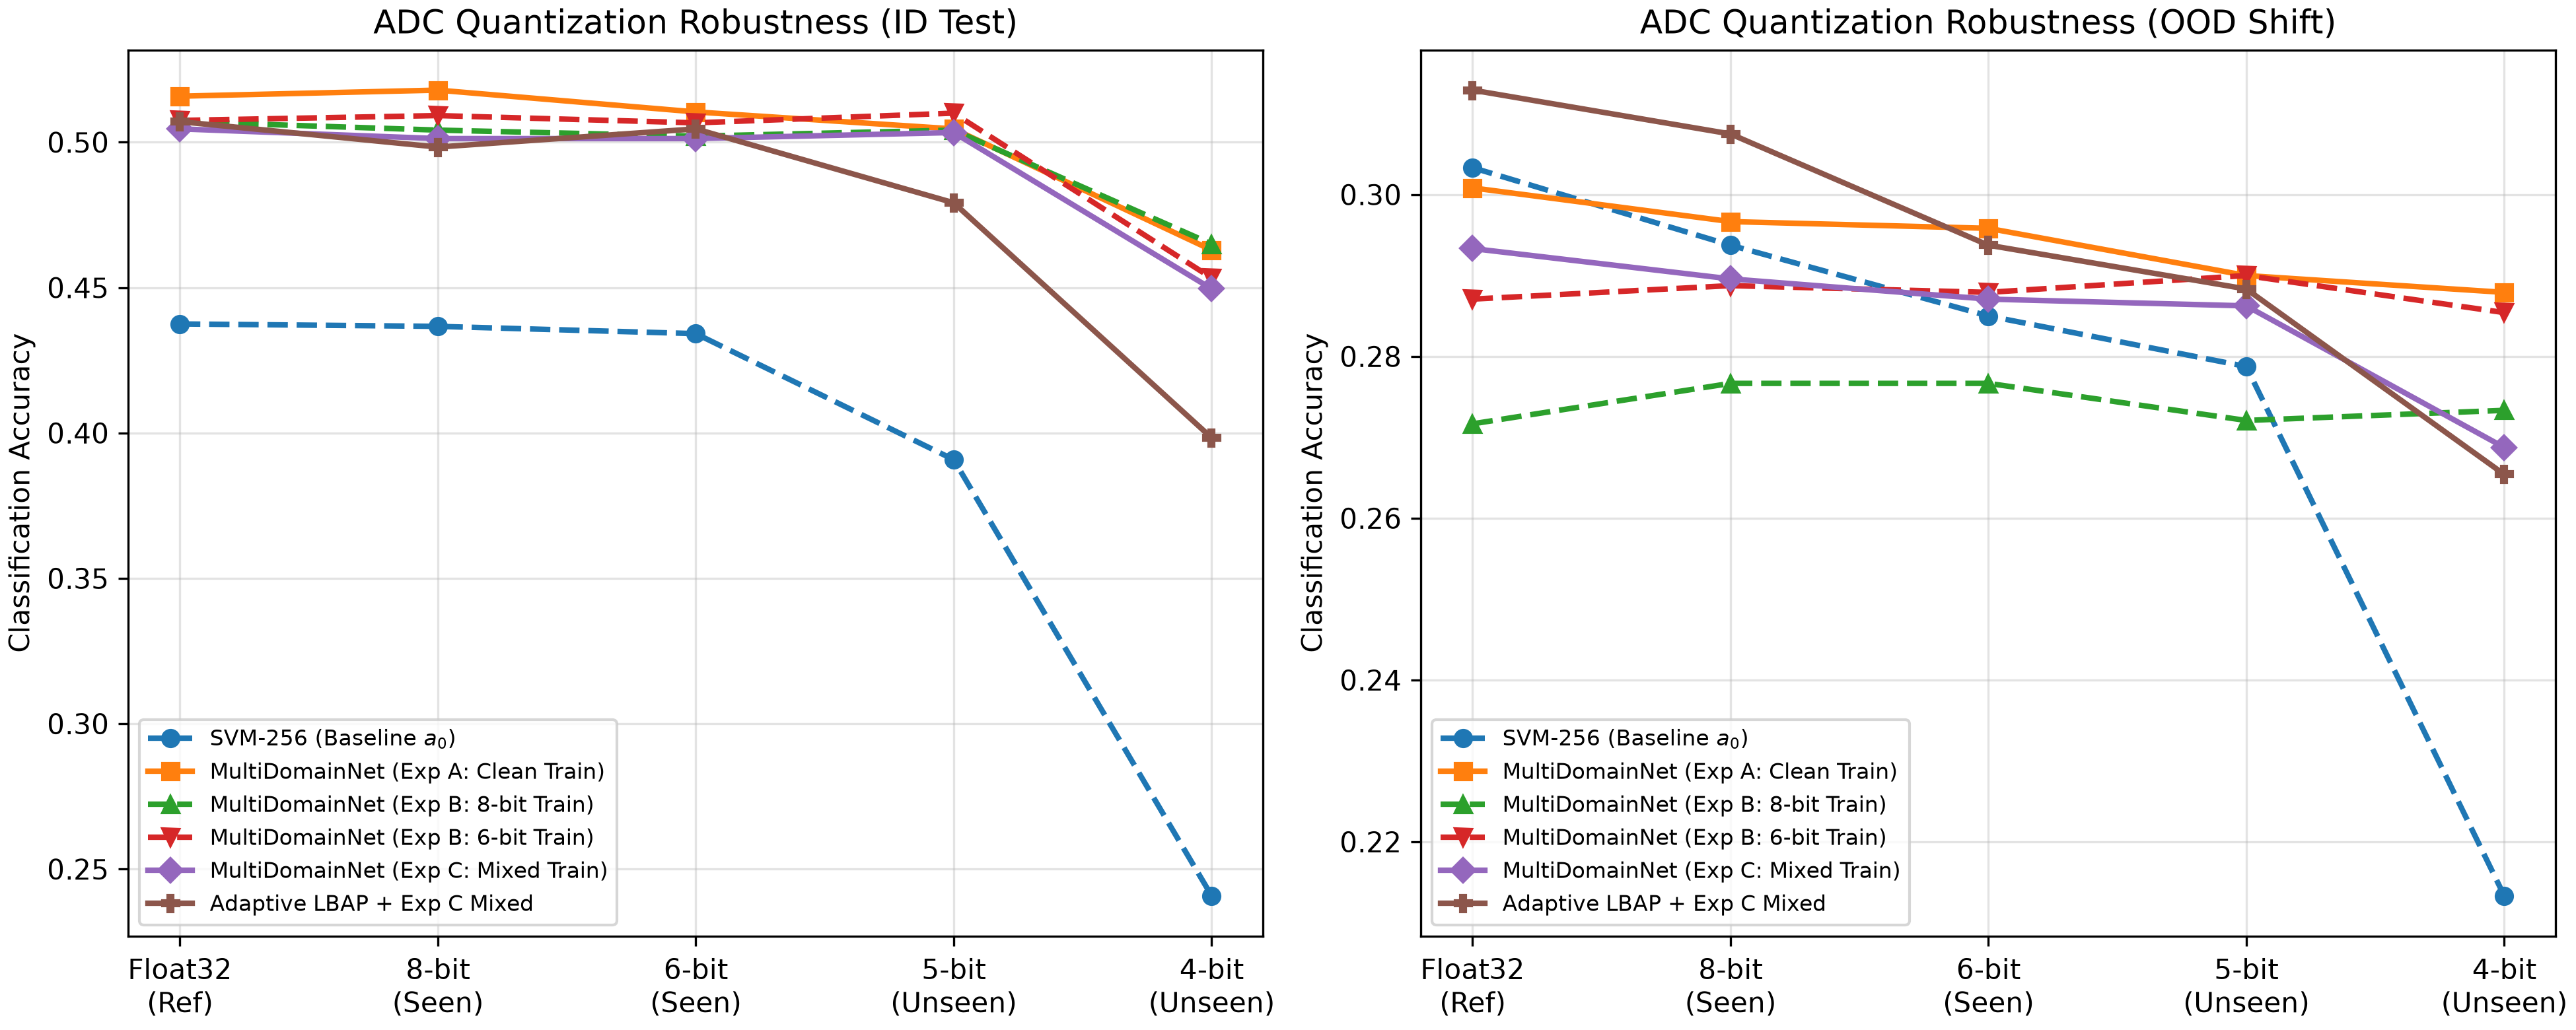
\includegraphics[width=\textwidth]{figures/fig3_adc_quantization_robustness.png}
\caption{Classification accuracy under virtual uniform mid-rise ADC quantization from floating-point down to $4$-bit resolution ($\mathrm{SQNR} = 7.87\,\mathrm{dB}$) on ID test (left) and OOD shift (right). MultiDomainAMCNet sustains $44.96\%$--$46.50\%$ accuracy at $4$ bits in-distribution, whereas conventional SVM classifiers collapse to $23.46\%$--$24.08\%$.}
\label{fig:adc_quantization_robustness}
\end{figure*}

\subsubsection{Probabilistic Uncertainty Calibration}
As reported in Panel~A of Table~\ref{tab:calibration_and_adc}, univariate Platt logistic regression fitted on validation margin scores successfully calibrates baseline $a_0$, driving in-distribution expected calibration error down to $\text{ECE}_{10} = 0.83\%$ ($\mathrm{NLL} = 0.6853$, $\mathrm{Brier} = 0.2461$).

For $\mathrm{MultiDomainAMCNet}$ ($a_2$), post-hoc temperature scaling optimizes $T^* = 0.9171$, reducing in-distribution calibration error from $2.90\%$ to $2.42\%$ and trimming Brier score to $0.1384$. However, an honest scientific assessment reveals an important edge limitation: under out-of-distribution domain shift ($\texttt{test\_shift}$), temperature scaling slightly \emph{worsens} overconfidence, increasing $\text{ECE}_{10}$ from $12.38\%$ (uncalibrated) to $13.82\%$ ($T^* = 0.9171$). Because $T^* < 1.0$, logits are sharpened to match in-distribution sharpness; when confronted with severe OOD channel dispersion, this sharpening slightly amplifies confidence on incorrect predictions. This demonstrates that scalar temperature scaling optimized in-distribution is insufficient for OOD channels, motivating domain-aware calibration in future work.

\subsubsection{Virtual ADC Quantization Breakdown}
To evaluate hardware suitability for low-power edge front-ends, baseband bursts undergo mid-rise uniform ADC quantization across $B \in \{\infty, 8, 6, 5, 4\}$ bits under fixed full-scale $V_{\mathrm{FS}} = 2.5\,\mathrm{V}$. Because fixed clipping ($5.12\%$ I/Q clip rate and $8.67\%$ sample saturation) dominates dynamic range distortion across $8$--$5$ bits, offline SQNR clusters around $8.51$--$8.24\,\mathrm{dB}$ before falling to $\mathrm{SQNR} = 7.87\,\mathrm{dB}$ at $4$-bit depth.

Under this coarse quantization:
\begin{itemize}
    \item Conventional SVM baselines suffer severe collapse: $\mathrm{SVM}_{256}$ drops from $43.75\%$ (FP32) to $24.08\%$ accuracy and $21.04\%$ macro F1 ($-19.67\,\mathrm{pp}$), approaching random-guess parity ($16.67\%$). $\mathrm{SVM}_{512}$ drops similarly to $23.46\%$ accuracy. Handcrafted cumulant estimators exhibit high sensitivity to harmonic distortion introduced by coarse quantization clipping.
    \item Conversely, all $\mathrm{MultiDomainAMCNet}$ neural variants maintain substantially higher accuracy than SVMs at $4$ bits ($44.96\%$ to $46.50\%$ vs.\ $23.46\%$--$24.08\%$ for SVMs). Crucially, however, mixed-resolution training (\texttt{Exp C}, $\{\infty, 8, 6\}$ bits) yields a \textbf{negative empirical outcome} at unseen $4$-bit quantization ($44.96\%$ accuracy, $46.62\%$ F1), underperforming clean \texttt{Exp A} training ($46.29\%$ accuracy, $48.80\%$ F1; $\Delta = -1.33\,\mathrm{pp}$) as well as fixed $8$-bit \texttt{Exp B8} ($46.50\%$). Fixed $6$-bit \texttt{Exp B6} achieves the highest $5$-bit accuracy ($51.00\%$) and highest $4$-bit OOD macro-F1 ($30.09\%$), whereas \texttt{Exp C} fails to generalize better than clean float32 training under unseen truncation+clipping ($5.12\%$ I/Q clip rate).
    \item \textbf{Router Gating Sensitivity:} Fast LBAP accuracy drops to $40.88\%$ (with Exp~A) and $39.83\%$ (with Exp~C) at $4$ bits. This reveals an important architectural insight: because the LBAP gating vector $\mathbf{g}(\mathbf{r}_{256})$ incorporates the decision margin of $\mathrm{SVM}_{256}$, the quantization-induced collapse of SVM features distorts gating predictions, artificially suppressing escalation. Resolving this requires training the prefix gating router with quantization-aware features.
\end{itemize}
